\chapter{Cel pracy}
Celem projektu jest przedstawienie tematu automatów komórkowych - pozyskanie wiedzy na temat ich działania oraz zastosowania. Efektem realizacji jest zaprojektowanie aplikacji z interfejsem graficznym.

\chapter{Wprowadzenie}

\chapter{Opracowanie teoretyczne}

\chapter{Specyfikacja wewnętrzna}

Do stworzenia aplikacji zostało wykorzystane środowisko app designer w matlabie. 
Aplikacja zawiera 4 reguły – każda z nich posiada własną metodę. Metody te przyjmują parametr app, który pozwala na korzystanie z pozostałych komponentów programu. W ciele funkcji zostaje modyfikowana siatka GRID w nieskończonej funkcji for. Modyfikacja zależy od zadanych warunków, które są specyficzne dla konkretnej reguły. Wynik jest prezentowany graficznie – przedstawienie siatki GRID.

\chapter{Specyfikacja zewnętrzna}

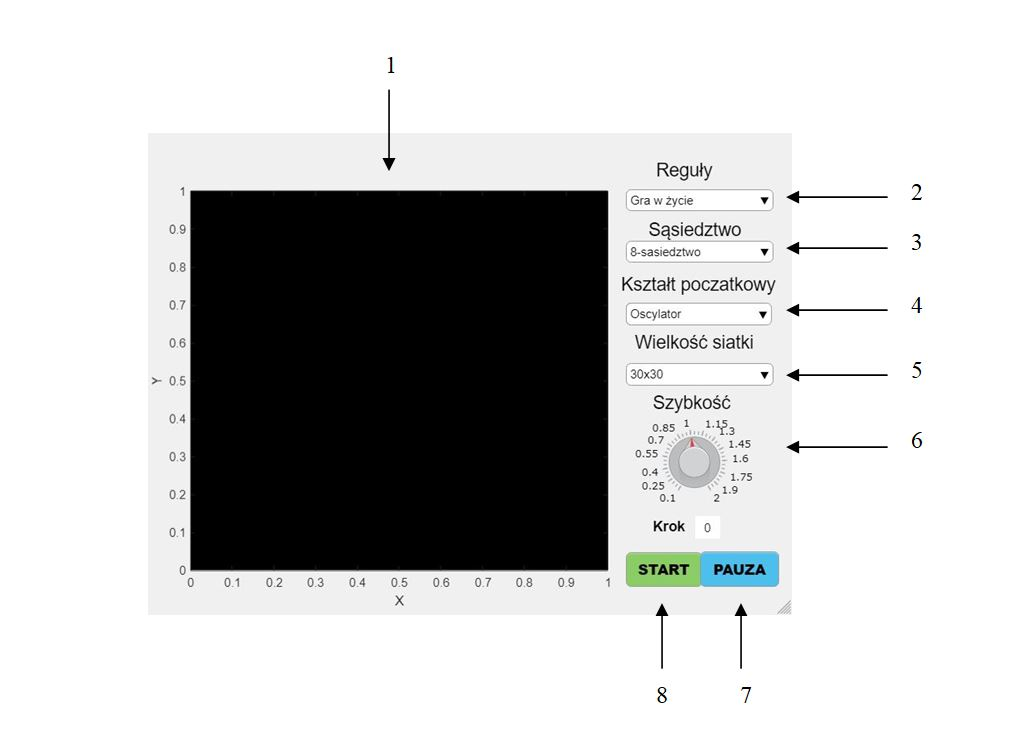
\includegraphics[scale=0.6]{zd}





\chapter{Wyniki}
\chapter{Podsumowanie}
